\documentclass[aspectratio=169,11pt]{beamer}

% ============================================================
% PACKAGES
% ============================================================
\usepackage{graphicx}
\usepackage{tikz}
\usetikzlibrary{positioning,arrows.meta}
\usepackage{xcolor}
\usepackage{booktabs}
\usepackage{tabularx}
\usepackage{array}
\usepackage{ragged2e}
\usepackage{hyperref}

% ============================================================
% COLORS - SAME AS PHASE-I
% ============================================================
\definecolor{GEUBlue}{RGB}{20,55,105}
\definecolor{GEULightBlue}{RGB}{238,244,251}
\definecolor{GEUGrey}{RGB}{90,90,90}
\definecolor{GEULightGrey}{RGB}{245,246,248}

% ============================================================
% BEAMER SETTINGS
% ============================================================
\usetheme{default}
\setbeamertemplate{navigation symbols}{}
\setbeamertemplate{blocks}[rounded][shadow=false]

\setbeamercolor{normal text}{fg=black,bg=white}
\setbeamercolor{frametitle}{fg=GEUBlue}
\setbeamercolor{structure}{fg=GEUBlue}
\setbeamercolor{block title}{fg=GEUBlue,bg=GEULightBlue}
\setbeamercolor{block body}{fg=black,bg=GEULightBlue}

\setbeamerfont{frametitle}{size=\Large,series=\bfseries}

% ============================================================
% LOGO
% ============================================================
% Upload Graphic Era logo as graphicera_logo.png
\newcommand{\GEULogo}{geu.png}

% ============================================================
% HEADER
% ============================================================
\setbeamertemplate{headline}{%
  \begin{tikzpicture}[remember picture,overlay]
    \node[
        anchor=north east,
        xshift=-0.30cm,
        yshift=-0.12cm
    ] at (current page.north east)
    {\includegraphics[height=0.62cm]{\GEULogo}};
  \end{tikzpicture}
  \vspace{0.72cm}
}

% ============================================================
% FRAME TITLE
% ============================================================
\setbeamertemplate{frametitle}{%
  \vspace{0.03cm}
  \insertframetitle\par
  \vspace{0.04cm}
  \textcolor{GEUBlue}{\rule{\textwidth}{0.9pt}}
  \vspace{0.03cm}
}

% ============================================================
% FOOTER
% ============================================================
\setbeamertemplate{footline}{%
  \leavevmode
  \hbox{%
  \begin{beamercolorbox}[
      wd=.82\paperwidth,
      ht=0.32cm,
      dp=0.10cm,
      leftskip=.3cm
  ]{author in head/foot}
    \tiny Department of Computer Science \& Engineering |
    Graphic Era (Deemed to be University)
  \end{beamercolorbox}%
  \begin{beamercolorbox}[
      wd=.18\paperwidth,
      ht=0.32cm,
      dp=0.10cm,
      rightskip=.3cm
  ]{date in head/foot}
    \hfill\tiny\insertframenumber/\inserttotalframenumber
  \end{beamercolorbox}}
}

% ============================================================
% CUSTOM COMMANDS
% ============================================================
\newcommand{\smallnote}[1]{%
\vspace{0.08cm}
{\scriptsize\color{GEUGrey}#1}
}

\newcommand{\placeholder}[1]{%
\textit{\color{GEUGrey}#1}
}

% ============================================================
% DOCUMENT INFORMATION
% ============================================================
\title{\textbf{Project-Based Learning}\\[2mm]\large Phase-III Evaluation}

\author{
\textbf{Project Title}\\
Team ID: XXXX
}

\institute{
Department of Computer Science \& Engineering\\
Graphic Era (Deemed to be University), Dehradun
}

\date{Academic Session 2026--27}

% ============================================================
% DOCUMENT
% ============================================================
\begin{document}

% ============================================================
% SLIDE 1
% ============================================================
\begin{frame}[plain]

\begin{tikzpicture}[remember picture,overlay]

\draw[GEUBlue,line width=3pt]
(current page.north west) -- (current page.north east);

\node[
    anchor=north east,
    xshift=-0.45cm,
    yshift=-0.35cm
] at (current page.north east)
{\includegraphics[height=1.0cm]{geu.png}};

\node[
    align=center,
    text width=.84\paperwidth
] at ([yshift=.25cm]current page.center)
{
{\color{GEUBlue}
\fontsize{26}{30}\selectfont
\bfseries PROJECT-BASED LEARNING}
\\[3mm]

{\fontsize{18}{22}\selectfont
PHASE-III FINAL EVALUATION}
\\[7mm]

{\color{GEUGrey}
\Large\bfseries
\placeholder{}}
\\[3mm]

{\color{GEUBlue}
\normalsize Team ID: DSCPP-III-2026-T170}
};

\node[
    align=center,
    anchor=south,
    yshift=.42cm
] at (current page.south)
{
\bfseries
Department of Computer Science \& Engineering\\
Graphic Era (Deemed to be University), Dehradun\\[-1mm]
\scriptsize Academic Session 2026--27
};

\end{tikzpicture}

\end{frame}

% ============================================================
% SLIDE 2
% ============================================================
\begin{frame}{Team \& Mentor Details}

\begin{columns}[T,totalwidth=\textwidth]

\column{.48\textwidth}

\begin{block}{Team Information}
\begin{tabular}{@{}ll@{}}
\textbf{Team ID:} DSCPP-III-2026-T170\\
\textbf{Semester:} 3rd \\
\textbf{Section:} ML2,DS1,DS2 \\
\textbf{Domain:} Machine Learning
\end{tabular}
\end{block}

\column{.48\textwidth}

\begin{block}{Team Members}
1.\quad \placeholder{Shubhangani Kotiyal -- 2510370294 – Team Leader}\\
2.\quad \placeholder{Ishanaya Agarwal -- 2510380249}\\
3.\quad \placeholder{Harshita Joshi -- 2510380118}\\
\end{block}

\end{columns}

\vspace{2mm}

\begin{block}{Mentor}
\placeholder{Dr. Hriday Kumar Gupta }
\hfill
\textbf{Interactions:}  \underline 3 {\hspace{12mm}}
\end{block}

\vfill


\end{frame}

% ============================================================
% SLIDE 3
% ============================================================
\begin{frame}{Project Abstract \& Problem Statement}

\begin{block}{Project Abstract}
ML-Core implements six machine learning algorithms in C++, emphasizing mathematical foundations and object-oriented programming.
\end{block}
\vspace{2mm}
\begin{block}{Problem Statement}
{
Our project implements machine learning algorithms in C++, demonstrating their mathematical foundations and computational mechanisms beyond pre-built libraries.
}
\end{block}
\vspace{2mm}
\textbf{\color{GEUBlue}Target Users / Application}
\begin{itemize}\itemsep2pt
    \item {Students learning the fundamentals of machine learning}
    \item {Educational institutions for practical demonstrations}
    \item {Learning and experimentation with mathematical models}
\end{itemize}

\smallnote{
Brief Discussion: Explain the problem and final solution in a concise
manner without repeating the complete Phase-I presentation.
}

\end{frame}

% ============================================================
% SLIDE 4
% ============================================================
\begin{frame}{Objectives \& Final Deliverables}

\begin{columns}[T,totalwidth=\textwidth]

\column{.48\textwidth}

\textbf{\color{GEUBlue}Finalized Objectives}

\begin{enumerate}\itemsep3pt
    \item {Implement six fundamental machine learning algorithms using C++}
    \item {Understand mathematical calculations behind each algorithm}
    \item {Apply object-oriented programming concepts}
    \item {Perform numerical computations and input validations}
    \item {Test and demonstrate implemented algorithms}
\end{enumerate}

\column{.48\textwidth}

\textbf{\color{GEUBlue}Final Deliverables}

\begin{itemize}\itemsep3pt
    \item {Six fundamental machine learning algorithms in C++}
    \item {Mathematical calculations behind each algorithm}
    \item {Object-oriented programming using separate classes}
    \item {Numerical computations and input validation}
    \item {Algorithm testing, demonstrations, and GitHub documentation}
\end{itemize}

\end{columns}

\vfill



\end{frame}

% ============================================================
% SLIDE 5
% ============================================================
\begin{frame}{Phase-I \& Phase-II Feedback Incorporated}

\scriptsize

\begin{center}

\renewcommand{\arraystretch}{1.35}

\begin{tabularx}{.96\textwidth}
{@{}p{2.1cm}X X@{}}

\toprule
\textbf{Phase} &
\textbf{Feedback / Suggestion} &
\textbf{Action Taken}\\
\midrule

Phase-I &
{Improve understanding of algorithmic calculations} &
{Implemented mathematical operations from scratch}\\

Phase-I &
{Organise the implementation into modules} &
{Created separate classes for six algorithms}\\

Phase-II &
{Improve data handling and validation} &
{Developed a common CSV loader with input validation}\\

Phase-II &
{Improve algorithm integration} &
{Developed a unified menu-driven application}\\

\bottomrule

\end{tabularx}

\end{center}

\vfill

\begin{block}{Final Improvement}
{
The project evolved from individual algorithm development into an integrated C++ application featuring reusable mathematical operations, modular architecture, CSV handling and algorithm execution.
}
\end{block}

\end{frame}

% ============================================================
% SLIDE 6
% ============================================================
\begin{frame}{Final System Architecture}

\begin{center}

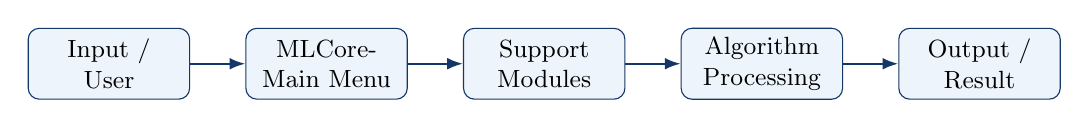
\begin{tikzpicture}[
node distance=7mm,
box/.style={
rectangle,
rounded corners,
draw=GEUBlue,
fill=GEULightBlue,
minimum width=2.05cm,
minimum height=9mm,
align=center,
font=\small
},
arrow/.style={
-{Latex[length=2mm]},
thick,
draw=GEUBlue
}
]

\node[box] (a) {Input /\\User};
\node[box,right=of a] (b) {MLCore- \\ Main Menu};
\node[box,right=of b] (c) {Support \\Modules};
\node[box,right=of c] (d) {Algorithm \\ Processing};
\node[box,right=of d] (e) {Output /\\Result};

\draw[arrow] (a)--(b);
\draw[arrow] (b)--(c);
\draw[arrow] (c)--(d);
\draw[arrow] (d)--(e);

\end{tikzpicture}

\end{center}

\vspace{4mm}

\begin{columns}[T,totalwidth=\textwidth]

\column{.48\textwidth}

\textbf{\color{GEUBlue}Major Components}

\begin{itemize}\itemsep2pt
    \item {MLCore:Manages menus and algorithm objects}
    \item {Dataset:Reads, validates and stores CSV data}
    \item {MathUtils:Provides reusable maths calculations}
    \item {Implement six Algorithm Modules}
\end{itemize}

\column{.68\textwidth}

\textbf{\color{GEUBlue}System Flow}

\begin{itemize}\itemsep2pt
    \item {User selects an algorithm from the menu}
    \item {Dataset loads and validates CSV data}
    \item {Algorithm processes data using MathUtils}
    \item {Results are displayed in the console}
\end{itemize}

\end{columns}

\vfill



\end{frame}

% ============================================================
% SLIDE 7
% ============================================================
\begin{frame}{Final Technology Stack}

\begin{columns}[T,totalwidth=\textwidth]

\column{.48\textwidth}

\begin{block}{Software / Technologies}
\begin{itemize}\itemsep2pt
    \item Programming: {C++}
    \item Framework: {Pure C++ Implementation}
    \item Database: {CSV Files}
    \item Libraries/APIs: {iostream, fstream, cmath}
    \item OS/Platform: {Local Console Application}
\end{itemize}
\end{block}

\column{.48\textwidth}

\begin{block}{Development Infrastructure}
\begin{itemize}\itemsep2pt
    \item IDE: {Visual Studio Code}
    \item Version Control: Git/GitHub
    \item Testing Tools: {Sample \& Edge-Case Testing}
    \item Deployment: {Local Execution}
    \item Other Tools: {CSV Datasets, README}
\end{itemize}
\end{block}

\end{columns}

\vfill



\end{frame}

% ============================================================
% SLIDE 8
% ============================================================
\begin{frame}{Implementation of PBL Course Concepts}

\scriptsize

\begin{center}

\renewcommand{\arraystretch}{1.25}

\begin{tabularx}{.96\textwidth}
{@{}>{\bfseries}p{2.8cm}X p{2.8cm}@{}}

\toprule
Course & Concepts Actually Implemented & Project Module\\
\midrule

Data Structures in C &
{Arrays, Sorting, Binary Trees, Recursion} &
{Dataset, KNN, Hierarchical Clustering}\\

OOPs with C++ &
{Classes, Objects, Encapsulation, Composition} &
{MLCore and Algorithm Classes}\\

\bottomrule

\end{tabularx}

\end{center}

\vfill

\begin{center}
\colorbox{GEULightBlue}{
\parbox{.88\textwidth}{
\centering
\textbf{Requirement:}
ML-Core requires a C++ compiler, standard libraries, CSV datasets, and an IDE supporting object-oriented programming, file handling, and mathematical computations
}}
\end{center}

\end{frame}

% ============================================================
% SLIDE 9
% ============================================================
\begin{frame}{Module-Wise Final Implementation}

\scriptsize

\begin{center}

\renewcommand{\arraystretch}{1.35}

\begin{tabularx}{.90\textwidth}
{@{}p{1.9cm}X p{2.4cm}p{2.4cm}@{}}

\toprule
\textbf{Module} &
\textbf{Implementation} &
\textbf{Responsible} &
\textbf{Status}\\
\midrule

{Linear Regression} &
{Least-squares prediction and MSE} &
{Shubhangani Kotiyal} &
Completed\\

{SVM} &
{Linear binary classification} &
{Ishanaya Agarwal} &
Completed\\

{KNN} &
{Distance calculation and majority voting} &
{Shubhangani Kotiyal} &
Completed\\

{K-means} &
{Two-cluster centroid-based grouping} &
{Ishanaya Agarwal} &
Completed\\

{Hierarchical Clustering} &
{Single-link clustering using binary trees} &
{Harshita Joshi} &
Completed\\

{PCA} &
{Data centering and dimensionality reduction} &
{Harshita Joshi} &
Completed\\

\bottomrule

\end{tabularx}

\end{center}

\vspace{4mm}

\begin{center}
\colorbox{GEULightBlue}{
\parbox{.65\textwidth}{
\centering
\textbf{Final Project Completion:}
\placeholder{100\%}
}}
\end{center}

\vfill

\end{frame}

% ============================================================
% SLIDE 10
% ============================================================
\begin{frame}{Working System / Prototype Demonstration}

\begin{columns}[T,totalwidth=\textwidth]

\column{.43\textwidth}

\textbf{\color{GEUBlue}Major Working Features}

\begin{itemize}\itemsep3pt
    \item {Integrated menu for six machine learning algorithms}
    \item {CSV-based numerical dataset loading}
    \item {Independent execution of algorithm modules}
    \item {Mathematical calculations without ML libraries}
    \item {Console-based predictions and results}
\end{itemize}

\column{.53\textwidth}

\begin{block}{System Screenshot / Output}

\centering
\vspace{2mm}

\includegraphics[width=\linewidth,height=3.2cm,keepaspectratio]{Screenshot 2026-11-22 at 10.11.41 PM.png}

\vspace{2mm}
\end{block}

\end{columns}

\vfill

\end{frame}

% ============================================================
% SLIDE 11
% ============================================================
\begin{frame}{Data / Database / Backend Implementation}

\begin{columns}[T,totalwidth=\textwidth]

\column{.48\textwidth}

\textbf{\color{GEUBlue}Data / Database}

\begin{itemize}\itemsep3pt
    \item {Data Source:Numerical CSV files}
    \item {Storage Structure: Fixed-size arrays}
    \item {Maximum Capacity: 100 rows}
    \item {Data Processing: Numerical validation and structured storage}
    \item {Retrieval: File input using fstream}
\end{itemize}

\column{.48\textwidth}

\textbf{\color{GEUBlue}Backend / Core Logic}

\begin{itemize}\itemsep3pt
    \item {MLCore manages algorithm execution}
    \item {Dataset handles CSV loading and validation}
    \item {MathUtils performs reusable mathematical calculations}
    \item {Six algorithm classes execute their respective operations}
    \item {Results are displayed through console output}
\end{itemize}

\end{columns}

\vfill

\end{frame}

% ============================================================
% SLIDE 12
% ============================================================
\begin{frame}{Testing \& Validation}

\scriptsize

\begin{center}

\renewcommand{\arraystretch}{1.35}

\begin{tabularx}{.96\textwidth}
{@{}p{2.0cm}X X p{1.4cm}@{}}

\toprule
Test Type &
Expected Result &
Observed Result &
Status\\
\midrule

{Compilation} &
{Successful compilation} &
{Compiled successfully} &
Pass\\

{Menu Testing} &
{All six options accessible} &
{Menu options verified} &
Pass\\

{CSV Validation} &
{Invalid input handled} &
{Selected CSV errors checked} &
Pass\\

{KNN Testing} &
{Correct neighbour selection} &
{Tie cases checked} &
Pass\\

{SVM Testing} &
{Consistent execution} &
{Repeated runs checked} &
Pass\\

{PCA Testing} &
{Valid projections} &
{Selected edge cases checked} &
Pass\\

\bottomrule

\end{tabularx}

\end{center}

\vspace{3mm}

\begin{block}{Validation Summary}
{
The project has successfully passed compilation checks, algorithm menu verification, sample execution and selected edge-case testing.
}
\end{block}

\end{frame}

% ============================================================
% SLIDE 13
% ============================================================
\begin{frame}{Results \& Performance Analysis}

\begin{columns}[T,totalwidth=\textwidth]

\column{.58\textwidth}

\textbf{\color{GEUBlue}Key Results}

\begin{itemize}\itemsep3pt
    \item {Linear Regression:Predictions and train MSE}
    \item {KNN:Nearest neighbours and predicted class labels}
    \item {K-Means:Cluster and centroid calculations}
    \item {SVM:Binary predictions and training accuracy}
    \item {Hierarchical Clustering:Single-link merge hierarchy}
    \item {PCA:Principal component projections and variance}
\end{itemize}

\column{.48\textwidth}

\begin{block}{Graph / Result Evidence}

\centering
\vspace{2mm}

\includegraphics[width=\linewidth,height=3.2cm,keepaspectratio]{Screenshot 2026-11-22 at 10.22.52 PM.png}

\vspace{2mm}

\end{block}

\end{columns}

\vfill

\end{frame}

% ============================================================
% SLIDE 14
% ============================================================
\begin{frame}{GitHub Repository \& Development Evidence}

\begin{columns}[T,totalwidth=\textwidth]

\column{.45\textwidth}

\textbf{\color{GEUBlue}Repository Details}

\begin{itemize}\itemsep3pt
    \item Repository: {https://github.com/Shubhangani-Kotiyal/PBL-ml-algorithms-in-c}
    \item Branch: {main}
    \item README.md: blob:https://github.com/201bb55f-c86a-4963-bde6-41e775e751c8
    \item Contributors: {All members}
    \item Documentation: {Available}
\end{itemize}

\column{.51\textwidth}

\textbf{\color{GEUBlue}Development Evidence}

\begin{itemize}\itemsep3pt
    \item {Regular commits}
    \item {Meaningful commit messages}
    \item {Individual commits}
    \item {Latest source code}
\end{itemize}

\end{columns}

\vfill

\end{frame}

% ============================================================
% SLIDE 15
% ============================================================
\begin{frame}{Individual Contribution}

\scriptsize

\begin{center}

\renewcommand{\arraystretch}{1.35}

\begin{tabularx}{.96\textwidth}
{@{}p{1.8cm}p{1.8cm}X p{1.5cm}@{}}

\toprule
Member &
Role &
Final Technical Contribution &
Commits\\
\midrule

{Shubhangani Kotiyal} &
{Team Leader} &
{Linear Regression and KNN} &
{20}\\

{Ishanaya Agarwal} &
{Developer} &
{SVM and K-means} &
{31}\\

{Harshita Joshi} &
{Developer} &
{Hierarchical Clustering and PCA} &
{19}\\

\bottomrule

\end{tabularx}

\end{center}

\vspace{3mm}

\begin{block}{Individual Evaluation}
Every member must be able to explain, demonstrate and defend
their individual technical contribution.
\end{block}

\end{frame}

% ============================================================
% SLIDE 16
% ============================================================
\begin{frame}{Challenges, Limitations \& Lessons Learned}

\begin{columns}[T,totalwidth=\textwidth]

\column{.58\textwidth}

\textbf{\color{GEUBlue}Challenges \& Solutions}

\begin{itemize}\itemsep3pt
    \item {Challenge1-Transition from C to C++:	Implementation OOPs concepts}
    \item {Challenge2-PCA calculations:Implemented eigenvalues and projections}
    \item {Challenge3-Hierarchical clustering:Used binary merge trees}
\end{itemize}

\vspace{2mm}

\textbf{\color{GEUBlue}Current Limitations}

\begin{itemize}\itemsep2pt
    \item {Fixed-size arrays limit datasets to 100 rows}
    \item {Broader validation is still pending}
\end{itemize}

\column{.48\textwidth}

\textbf{\color{GEUBlue}Technical Learning}

\begin{itemize}\itemsep3pt
    \item {Understanding mathematical foundations of ML algorithms}
    \item {Applying object-oriented programming}
    \item {Developing reusable maths modules}
\end{itemize}

\vspace{2mm}

\textbf{\color{GEUBlue}Team Learning}

\begin{itemize}\itemsep2pt
    \item {Collaborative software development}
    \item {Modular code organisation}
    \item {Debugging and problem-solving}
\end{itemize}

\end{columns}

\vfill

\end{frame}

% ============================================================
% SLIDE 17
% ============================================================
\begin{frame}{Final Outcomes, Applications \& Future Scope}

\begin{columns}[T,totalwidth=\textwidth]

\column{.32\textwidth}

\textbf{\color{GEUBlue}Final Outcomes}

\begin{itemize}\itemsep3pt
    \item {Six ML algorithms
    from scratch}
    \item {Modular C++ application}
    \item {Reusable maths and dataset modules}
\end{itemize}

\column{.38\textwidth}

\textbf{\color{GEUBlue}Applications}

\begin{itemize}\itemsep3pt
    \item {Educational demonstrations of ML algos}
    \item {Understanding regression and classification}
    \item {Exploring clustering and data reduction}
\end{itemize}

\column{.42\textwidth}

\textbf{\color{GEUBlue}Future Scope}

\begin{itemize}\itemsep3pt
    \item {Support larger datasets}
    \item {Implement multiclass and nonlinear classification}
    \item {Introduce graphical result visualization}
\end{itemize}

\end{columns}

\vspace{5mm}

\begin{block}{Tangible Project Outcome}
{
A working, menu-driven C++ application that demonstrates six fundamental machine learning algorithms through independently implemented mathematical operations.
}
\end{block}

\end{frame}

% ============================================================
% SLIDE 18
% ============================================================
\begin{frame}{References \& Project Resources}

\begin{columns}[T,totalwidth=\textwidth]

\column{.46\textwidth}

\textbf{\color{GEUBlue}References}

\begin{enumerate}\itemsep3pt
    \item {Christopher M. Bishop – Pattern Recognition and Machine Learning}
    \item {Gareth James et al. – An Introduction to Statistical Learning}
    \item {Andrew Ng – Machine Learning educational resources}
    \item {C++ Reference – Standard library documentation}
    \item {ML algorithm mathematical references}
\end{enumerate}

\column{.53\textwidth}

\textbf{\color{GEUBlue}Project Resources}

\begin{itemize}\itemsep3pt
    \item GitHub: {https://github.com/Shubhangani-Kotiyal/PBL-ml-algorithms-in-c}
    \item Demo: {NA}
    \item Dataset: {https://github.com/Shubhangani-Kotiyal/PBL-ml-algorithms-in-c/tree/724b7d9bed04e2bdd8e809036d1a4c895ebd955c/datasets}
    \item Documentation: {https://github.com/Shubhangani-Kotiyal/PBL-ml-algorithms-in-c/blob/724b7d9bed04e2bdd8e809036d1a4c895ebd955c/README.md}
\end{itemize}

\vfill

\begin{center}

\colorbox{GEUBlue}{
\parbox{.82\textwidth}{
\centering
\color{white}
\Large\textbf{Thank You}\\[1mm]
\normalsize Questions \& Discussion
}}

\end{center}

\end{columns}

\end{frame}

\end{document}
